%%% Template originaly created by Karol Kozioł (mail@karol-koziol.net) and modified for ShareLaTeX use

\documentclass[11pt]{article}
\usepackage{esvect}
\usepackage[T1]{fontenc}
\usepackage[utf8]{inputenc}
\usepackage{graphicx}
\usepackage{xcolor}
\usepackage{float}
\usepackage{tabto}
\usepackage{bm}
\usepackage{tgtermes}
\usepackage{natbib}
%\usepackage[subnum]{cases}
\usepackage[super]{nth}
\bibpunct{(}{)}{;}{a}{}{,}
\usepackage{amsmath,amssymb}
\usepackage{enumerate}
\usepackage{multicol}
\usepackage{tikz}
\usepackage[amssymb]{SIunits}
\usepackage{rotating}
\usepackage{enumitem}
\usepackage{geometry}
\geometry{total={8.5in,11in},
left=1in,right=1in,%
bindingoffset=0mm, top=1in,bottom=1in}
\usepackage[super]{nth}
\usepackage[
pdftitle={EFD: Exam 1, in-class}, 
pdfauthor={Jeremy Gibbs, University of Utah},
colorlinks=true,linkcolor=blue,urlcolor=blue,citecolor=blue,bookmarks=true,
bookmarksopenlevel=2]{hyperref}

\linespread{1.1}
\setlength{\parskip}{1em}
\setlength{\parindent}{0pt}
\newcommand{\linia}{\rule{\linewidth}{0.5pt}}
\makeatletter
\renewcommand{\maketitle}{
\begin{center}
\vspace{2ex}
{\huge \textsc{\@title}}
\vspace{1ex}
\\
\linia\\
ME EN 7710 \hfill Exam \#1 \hfill In-Class Portion
\vspace{4ex}
\end{center}
}
\makeatother
%%%

% custom footers and headers
\usepackage{fancyhdr,lastpage}
\pagestyle{fancy}
\lhead{}
\chead{}
\rhead{}
%\lfoot{Assignment \textnumero{} 5}
\cfoot{}
\rfoot{Page \thepage~/~\pageref*{LastPage}}
\renewcommand{\headrulewidth}{0pt}
\renewcommand{\footrulewidth}{0pt}
%

%%%----------%%%----------%%%----------%%%----------%%%

\begin{document}

\title{Environmental Fluid Dynamics}

\maketitle

%-- Question 1 --%
\vspace{-20pt}
\paragraph{1.) [10 points] Matching}~\\
\begin{enumerate}
	\begin{minipage}{0.4\linewidth}
    \item[] $\rule{1cm}{0.15mm}$ isotropic
    \item[] $\rule{1cm}{0.15mm}$ flux divergence
    \item[] $\rule{1cm}{0.15mm}$ specific humidity
    \item[] $\rule{1cm}{0.15mm}$ thermal diffusivity
    \item[] $\rule{1cm}{0.15mm}$ mixing ratio
	\end{minipage}
	\begin{minipage}{0.6\linewidth}
    \item ratio of mass of water vapor to mass of dry air
    \item invariant to rotation and reflection
    \item invariant to spatial translation
    \item ratio of thermal conductivity to heat capacity
    \item the ability of a material to conduct heat
    \item cooling of a layer due to change in net radiation with height
    \item ratio of mass of water vapor to mass of moist air
    \item time, ensemble, and space averages are equal
	\end{minipage}
\end{enumerate}

%-- Question 2 --%
\paragraph{2.) [6 points] Consider a very thin, no mass, no heat capacity surface, under typical clear sky conditions. Indicate the signs of the following heat fluxes (assume a sign convention where fluxes leaving the surface are positive)}
\begin{enumerate}[label=\alph*.)]
	\item Ground heat flux during the night:\tabto{6cm} $\rule{1cm}{0.15mm}$
	\item Sensible heat flux during the day:\tabto{6cm} $\rule{1cm}{0.15mm}$
	\item Latent heat flux during the night:\tabto{6cm} $\rule{1cm}{0.15mm}$
\end{enumerate}


%-- Question 3 --%
\paragraph{3.) [4 points] Again consider the simplified surface energy balance for thin, no mass, no heat capacity surface, under typical clear sky conditions. Provide one reason why this balance might be unsatisfactory for an urban neighborhood?}

%-- Question 4 --%
\paragraph{4.) [6 points] Describe the following dimensionless numbers using words or equations.}
\begin{enumerate}[label=\alph*.)]
\item Rossby Number
\vspace{20pt}
\item Bowen Ratio
\vspace{20pt}
\item Ekman Number
\end{enumerate}

%-- Question 5 --%
\paragraph{5.) [8 points] Sketch and label the vertical temperature profiles for an (a) adiabatic, (b) superadiabatic, (c) subadiabatic, and (d) isothermal atmosphere.}~\\

\vspace{225pt}

%-- Question 6 --%
\paragraph{6.) [4 points] What phenomena does this figure illustrate? What is its interpretation?.}~\\
\begin{figure}[H]
	\centering
	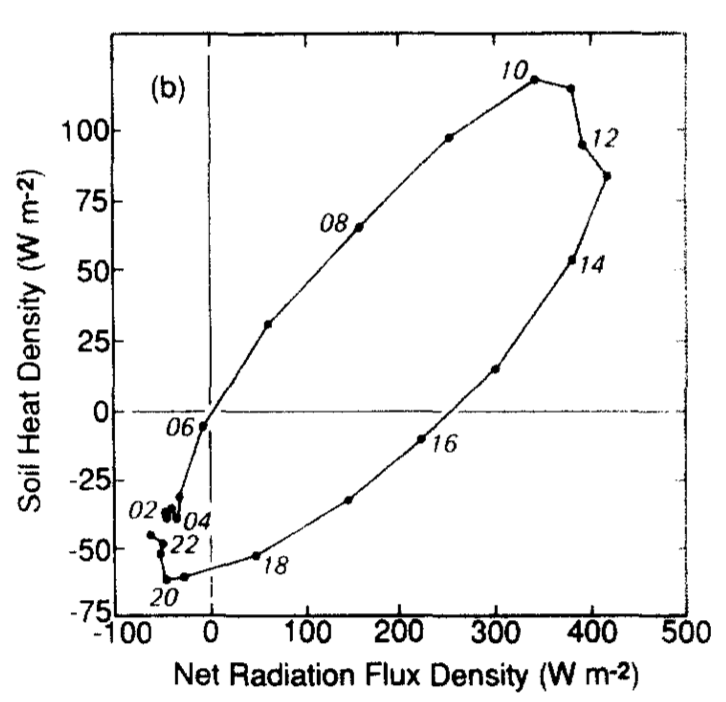
\includegraphics[width=0.55\textwidth]{fig1}
\end{figure}

\newpage
%-- Question 7 --%
\paragraph{7.) [12 points] Ekman Layer}~\\
\begin{enumerate}[label=\alph*.)]
\item Sketch the hodograph of the Ekman layer solution above a rigid surface.
\vspace{225pt}
\item Sketch the vertical profiles of the horizontal momentum components for the Ekman layer solution above a rigid surface.
\vspace{225pt}
\item What is Ekman pumping?
\end{enumerate}
\newpage

%-- Question 8 --%
\paragraph{8.) [16 points] Scale Analysis}
\begin{enumerate}[label=\alph*.)]
\item ~[5 points] Using characteristic values for the synoptic scale (located on the provided equation sheet), perform scale analysis of the following horizontal equation of motion.
$$\frac{\partial u}{\partial t} + u \frac{\partial u}{\partial x} + v \frac{\partial u}{\partial y}+ w \frac{\partial u}{\partial z} = - \frac{1}{\rho} \frac{\partial p}{\partial x} + fv + \nu\left(\frac{\partial^2 u}{\partial x^2} + \frac{\partial^2 u}{\partial y^2} + \frac{\partial^2 u}{\partial z^2}\right)$$
\vspace{130pt}
\item ~[3 points] Which approximation may be used to describe the horizontal flow based on the dominant terms above? Be sure to describe the relevant balance of forces.
\vspace{55pt}
\item ~[5 points] Repeat the scale analysis of the following vertical equation of motion using characteristic values for the synoptic scale.
$$\frac{\partial w}{\partial t} + u \frac{\partial w}{\partial x} + v \frac{\partial w}{\partial y}+ w \frac{\partial w}{\partial z} = - \frac{1}{\rho} \frac{\partial p}{\partial z} - g + \nu\left(\frac{\partial^2 w}{\partial x^2} + \frac{\partial^2 w}{\partial y^2} + \frac{\partial^2 w}{\partial z^2}\right)$$
\vspace{130pt}
\item ~[3 points] Which approximation may be used to describe the vertical flow based on the dominant terms above? Be sure to describe the relevant balance of forces.
\end{enumerate}
\newpage

%-- Question 9 --%
\paragraph{9.) [5 points] Using the provided Coriolis term that we derived for the mechanical energy equation, show the work done by the Coriolis force.}

$$\vv{U} \cdot \left(-2\rho \vv{\Omega} \times \vv{U} \right) = \epsilon_{ij3}fu_iu_j$$
\vspace{150pt}

%-- Question 10 --%
\paragraph{10.) [3 points] What are the three typical approaches to studying turbulence?}
\begin{enumerate}[label=\alph*.)]
\item $\rule{7cm}{0.15mm}$
\vspace{10pt}
\item $\rule{7cm}{0.15mm}$
\vspace{10pt}
\item $\rule{7cm}{0.15mm}$
\end{enumerate}

%-- Question 11 --%
\paragraph{11.) [3 points] Name three characteristics of turbulence.}
\begin{enumerate}[label=\alph*.)]
\item $\rule{7cm}{0.15mm}$
\vspace{10pt}
\item $\rule{7cm}{0.15mm}$
\vspace{10pt}
\item $\rule{7cm}{0.15mm}$
\end{enumerate}

%-- Question 12 --%
\paragraph{12.) [3 points] What is meant by the ergodic condition?}~\\
\newpage

%-- Question 13 --%
\paragraph{13.) [14 points] Taylor-Proudman Theorem}~\\
\begin{enumerate}[label=\alph*.)]
\item ~[10 points] Starting with the simplified equations of motion for a rotating, inviscid, homogeneous fluid, derive the Taylor-Proudman outcome of $\partial \vv{U}/\partial z=0$
$$-2\Omega v = -\frac{1}{\rho}\frac{\partial p}{\partial x}\quad (1)\qquad 
		2\Omega u = -\frac{1}{\rho}\frac{\partial p}{\partial y}\quad (2)\qquad
		0 = -\frac{1}{\rho}\frac{\partial p}{\partial z} -g\quad (3)$$
\vspace{300pt}
\item ~[4 points] Explain one implication of the theorem.
\end{enumerate}
\newpage

%-- Question 14 --%
\paragraph{14.) [6 points] Consider the following equation for the internal energy ($I$, we also wrote this as $e$) at a point in the atmosphere. We derived this as part of the thermal energy equation. Provide a physical meaning for each term.}

$$\underbrace{\rho \frac{DI}{Dt}}_{1} = \underbrace{\vphantom{\frac{DI}{Dt}}-\vv{\nabla}\cdot \vv{q}}_{2} -\underbrace{\vphantom{\frac{DI}{Dt}}\vv{\nabla}\cdot (p\vv{U})}_{3} \underbrace{\vphantom{\frac{DI}{Dt}}-\vv{\nabla}\cdot \vv{R_n}}_{4} + \underbrace{\vphantom{\frac{DI}{Dt}}L_v\epsilon}_{5} + \underbrace{\vphantom{\frac{DI}{Dt}}\mu \Phi_\nu}_{6}$$
\vspace{20pt}
\begin{enumerate}
\item $\rule{10cm}{0.15mm}$
\vspace{10pt}
\item $\rule{10cm}{0.15mm}$
\vspace{10pt}
\item $\rule{10cm}{0.15mm}$
\vspace{10pt}
\item $\rule{10cm}{0.15mm}$
\vspace{10pt}
\item $\rule{10cm}{0.15mm}$
\vspace{10pt}
\item $\rule{10cm}{0.15mm}$
\end{enumerate}

\newpage
\paragraph{Potentially Useful Information}~\\

\textbf{Characteristic Values for the Synoptic Scale}
\begin{itemize}
\begin{minipage}{0.35\linewidth}
\item $\nu \sim 10^-5\ \metre\squared\ \reciprocal\second$
\item $V \sim 10\ \metre\reciprocal\second$
\item $W \sim 0.1\ \metre\reciprocal\second$
\item $L \sim 1000\ \kilo\metre = 10^6\ \metre$
\item $H \sim 10\ \kilo\metre = 10^4\ \metre$
\end{minipage}
\begin{minipage}{0.65\linewidth}
\item $T \sim L/V \sim 10^5\ \second$
\item $f \sim 10^{-4}\ \reciprocal\second$
\item $\rho \sim 1\ \kilo\gram \, \rpcubic\metre$
\item $\Delta p$ in horizontal $\sim 10\ \milli\barn = 1000\ \pascal$
\item $\Delta p$ over vertical length scale $H \sim 1000\ \milli\barn = 10^5\ \pascal$
\end{minipage}
\end{itemize}

\textbf{Tensors}

\begin{align*}
\delta_{mn} &= 
	\begin{cases}
    +1, & \text{if } m=n\\
    0   & \text{if } m \neq n
	\end{cases}\\
	\epsilon_{mnq} &= 
	\begin{cases}
    +1, & \text{if } mnq = 123, 231, 312\quad \text{even permutation}\\
    -1  & \text{if } mnq = 321, 213, 132\quad \text{odd permutation}\\
    0   & \text{if } m=n, n=q, q=m\quad \text{any two indices repeated}
	\end{cases}
\end{align*}
	
	
	
	
	
	
	
	
	
	
	
	
	
\end{document}